\documentclass[12pt,a4paper]{report}

%---------------------------------------------------------------
% B.Tech project report. Compile with pdfLaTeX twice.
% Figures expected in ./figures/ :
%   df2_df4_newtonian.png, df44_stellar_only.png,
%   df44_nfw_bestfit.png, df44_nfw_fit_residuals.png
%---------------------------------------------------------------
\usepackage[a4paper,top=1in,bottom=1in,left=1.3in,right=1in]{geometry}
\usepackage[T1]{fontenc}
\usepackage[utf8]{inputenc}
\usepackage{times}
\usepackage{amsmath,amssymb}
\usepackage{graphicx}
\usepackage{booktabs,array}
\usepackage{setspace}
\usepackage{fancyhdr}
\usepackage{hyperref}
\usepackage{xcolor}
\usepackage{caption}
\usepackage{float}
\usepackage{microtype}
\usepackage{enumitem}
\graphicspath{{figures/}}
\onehalfspacing
\setlength{\headheight}{16pt}
\setlength{\parindent}{1.2em}
\setlength{\parskip}{0pt}
% Chapters are numbered. Major topics are sections (unnumbered, listed in the
% contents); minor topics are smaller headings (\subsection*, not listed).
\setcounter{secnumdepth}{0}
\setcounter{tocdepth}{1}
\numberwithin{equation}{chapter}
\hypersetup{colorlinks=true,linkcolor=black,citecolor=black,urlcolor=blue,
            pdftitle={Probing Dark Matter in Ultra-Diffuse Galaxies Using Velocity Dispersion}}

%===============================================================
% PERSONAL DETAILS
%===============================================================
\newcommand{\thesistitle}{Probing Dark Matter in Ultra-Diffuse Galaxies Using Velocity Dispersion}
\newcommand{\authorname}{Shivasheesh}
\newcommand{\rollnumber}{230121051}
\newcommand{\guidename}{Dr. Sovan Chakraborty and Dr. Sayan Chakrabarti}
\newcommand{\department}{Department of Physics}
\newcommand{\institute}{Indian Institute of Technology Guwahati}
\newcommand{\instituteaddress}{Guwahati -- 781039, Assam}
\newcommand{\thesisyear}{2026}
%===============================================================

\pagestyle{fancy}
\fancyhf{}
\fancyhead[L]{\small\textit{Dark matter in ultra-diffuse galaxies}}
\fancyhead[R]{\small\textit{\authorname}}
\fancyfoot[C]{\thepage}
\renewcommand{\headrulewidth}{0.4pt}

\begin{document}
\pagenumbering{gobble}
\begin{titlepage}
\begin{center}
\vspace*{1.2cm}
{\LARGE\bfseries\thesistitle\par}
\vspace{1.8cm}
{\large\itshape A B.Tech Project Report Submitted\\[0.25cm]
in Partial Fulfilment of the Requirements\\[0.25cm]
for the Degree of\par}
\vspace{0.5cm}
{\large\bfseries Bachelor of Technology\par}
\vspace{0.9cm}
{\large\itshape by\par}
\vspace{0.25cm}
{\Large\bfseries\authorname\par}
\vspace{0.2cm}
{\large (\rollnumber)\par}
\vspace{0.7cm}
{\large\itshape under the guidance of\par}
\vspace{0.25cm}
{\large\bfseries\guidename\par}
\vspace{0.75cm}
\IfFileExists{logoo.eps}{\includegraphics[width=3.5cm]{logoo.eps}}{\vspace{1.4cm}}
\vfill
{\large\bfseries\MakeUppercase{\department}\\[0.25cm]
\MakeUppercase{\institute}\\[0.25cm]
\instituteaddress\\[0.5cm]
\thesisyear\par}
\end{center}
\end{titlepage}

%---------------------------------------------------------------
% Certificate
%---------------------------------------------------------------
\clearpage
\pagenumbering{roman}
\setcounter{page}{1}

\chapter*{Certificate}
\addcontentsline{toc}{chapter}{Certificate}
\vspace{0.9cm}

This is to certify that the project report entitled
\textbf{``\thesistitle''}, submitted by \textbf{\authorname}
(Roll No. \rollnumber) to the \department, \institute,
in partial fulfilment of the requirements for the degree of
Bachelor of Technology, presents work carried out under our guidance
and supervision.

\vspace{0.7cm}
This report has been prepared for academic evaluation as part of the
B.Tech project requirements. To the best of our knowledge, the work
reported here has not been submitted elsewhere for the award of a degree
or diploma.

\vspace{0.5cm}
\vfill
\noindent Date: \rule{4cm}{0.4pt}\hfill Place: Guwahati

\vspace{1.5cm}
\noindent
\begin{minipage}[t]{0.48\textwidth}
  \rule{5.5cm}{0.4pt}\\[0.2cm]
  \textbf{Dr. Sovan Chakraborty}\\[0.1cm]
  Supervisor\\
  \department\\
  \institute
\end{minipage}
\hfill
\begin{minipage}[t]{0.48\textwidth}
  \raggedleft
  \rule{5.5cm}{0.4pt}\\[0.2cm]
  \textbf{Dr. Sayan Chakrabarti}\\[0.1cm]
  Supervisor\\
  \department\\
  \institute
\end{minipage}

%---------------------------------------------------------------
% Acknowledgement
%---------------------------------------------------------------
\clearpage
\chapter*{Acknowledgement}
\addcontentsline{toc}{chapter}{Acknowledgement}
\vspace{0.7cm}

I would like to thank my project supervisors, Dr. Sovan Chakraborty and Dr. Sayan Chakrabarti, for the guidance
and feedback provided during this project. Our discussions helped me
understand the assumptions behind the dynamical models and clarify the
scope of the numerical calculations presented in this report.

I would also like to thank Dikshit Mahanta, a Ph.D. scholar at IIT Guwahati, for his support and guidance.

I am grateful to the \department, \institute, for providing the academic
environment and resources needed to carry out this work. I also thank
the researchers whose published studies and observational data made the
present computational replication possible.

Finally, I thank my friend Siddhanta for misinterpreting H1 with Hydrogen Iodide and making us all laugh.

\vfill
\begin{flushright}
\textbf{\authorname}\\
Roll No. \rollnumber\\
\department\\
\institute\\
\thesisyear
\end{flushright}

%---------------------------------------------------------------
% Abstract
%---------------------------------------------------------------
\clearpage
\chapter*{Abstract}
\addcontentsline{toc}{chapter}{Abstract}
Ultra-diffuse galaxies (UDGs) combine dwarf galaxies' stellar content with larger galaxy sizes, making their dark matter a critical aspect of dynamical modeling. This project investigates the line-of-sight velocity dispersion of three UDGs NGC1052-DF2, NGC1052-DF4, and Dragonfly 44 (DF44) to explore dark matter constraints. By employing Newtonian gravity and the spherical Jeans equation, the stellar mass distributions are converted into projected dispersion profiles for comparison with existing kinematics. DF2 and DF4 show stellar-only models in line with observed velocities, suggesting no dark matter presence. However, DF44's models do not match the measured dispersions, indicating a dark-matter dominated system fitting an NFW profile. The findings reveal degeneracies in halo mass, concentration, and anisotropy, pointing to tighter constraints on local mass than on overall halo attributes. This research highlights the strengths and limitations of velocity dispersion as a tool for probing dark matter in UDGs.

\vspace{0.4cm}
\noindent\textbf{Keywords:} ultra-diffuse galaxies; dark matter; stellar kinematics; Newtonian gravity; Jeans equation; velocity anisotropy; NFW halo.

\clearpage
\tableofcontents
\clearpage
\listoffigures
\clearpage
\chapter*{List of Symbols and Abbreviations}
\addcontentsline{toc}{chapter}{List of Symbols and Abbreviations}
\begin{tabular}{@{}p{3.0cm}p{10.0cm}@{}}
\toprule
\textbf{Symbol} & \textbf{Meaning} \\
\midrule
UDG & Ultra-diffuse galaxy \\
GC & Globular cluster \\
LOS & Line of sight \\
NFW & Navarro--Frenk--White halo profile \\
$r$; $R$ & Three-dimensional radius; projected radius on the sky \\
$\nu(r)$ & Three-dimensional tracer luminosity or number density \\
$\rho(r)$ & Gravitating mass density \\
$M(r)$ & Total mass enclosed within radius $r$ \\
$\Phi(r)$ & Newtonian gravitational potential \\
$\sigma_r(r)$ & Radial velocity dispersion \\
$\sigma_{\rm LOS}(R)$ & Line-of-sight velocity dispersion \\
$\beta$ ($\xi$) & Velocity anisotropy parameter (the DF44 paper uses $\xi$) \\
$\Upsilon_\star$ & Stellar mass-to-light ratio \\
$R_e$; $n$ & Effective radius; S\'ersic index \\
$r_{1/2}$ & Three-dimensional half-light radius \\
$a_\star$; $\rho_0$ & Scale radius and surface-density scale of the DF2/DF4 stellar profile \\
$r_s$; $\rho_s$ & NFW scale radius; NFW scale density \\
$M_{200}$; $c$ & Halo mass within $r_{200}$; halo concentration \\
$\chi^2$; $N$; $k$ & Fit statistic; number of data points; number of free parameters \\
\bottomrule
\end{tabular}

\clearpage
\pagenumbering{arabic}
\setcounter{page}{1}

%===============================================================
\chapter{Introduction}
%===============================================================

\section{Motivation}

Ultra-diffuse galaxies (UDGs) have low surface brightness despite having sizes comparable to those of substantially more luminous galaxies. Their dynamical masses are therefore of particular interest: a faint stellar component does not necessarily imply a weak gravitational field. The motions of stars or globular clusters provide an observational route to the matter distribution, although the inferred mass depends on assumptions about geometry and orbital structure.

NGC1052-DF2 and NGC1052-DF4 are two widely discussed systems whose measured globular-cluster velocities permit models with little additional dark matter under the adopted distance and equilibrium assumptions \cite{vandokkum2018,vandokkumdf4_2019}. Dragonfly~44, a UDG in the Coma cluster, represents a contrasting case. Spatially resolved stellar spectroscopy reveals a substantially larger line-of-sight velocity dispersion, and dark matter contributes significantly in conventional dynamical models \cite{vandokkumdf44_2019}. The interpretation of these systems has evolved with observational updates; they are therefore treated here as contrasting modelling cases rather than definitive evidence for or against dark matter in all UDGs.

Bhatia, Chakrabarti, and Chakraborty studied DF2 and DF4 using Newtonian and modified gravitational models \cite{bhatia2023}. A later study investigated anisotropy and alternative gravity in DF44 and compared those descriptions against an NFW halo \cite{bhatia2024}. The present project concentrates on the Newtonian baselines relevant to Fig.~1 of each of these papers. The modified-gravity prescriptions considered by the authors are not implemented here.

\section{Objectives and Scope}

The objective is to calculate line-of-sight velocity-dispersion profiles from specified spherical mass models and to test whether visible matter alone can account for the observed kinematics. The calculation follows a common sequence: a stellar density profile defines the enclosed mass, the mass supplies the Newtonian potential gradient in the Jeans equation, and the radial velocity dispersion is projected onto the observer's line of sight.

For DF2 and DF4, the stellar-only prediction is compared with globular-cluster velocities. For DF44, stellar-only predictions are compared with resolved stellar dispersions for several orbital anisotropies, and a Newtonian model with an NFW halo is then fitted to the data. The exercise replicates selected Newtonian calculations from the two source papers and provides an independent refit of the DF44 NFW halo under simpler constraints than those of the source study, with a physical discussion of what the data can and cannot constrain. All numerical work is carried out in Python with NumPy, SciPy and Matplotlib.

\subsection*{Organisation of the Report}

Chapter~2 develops the theoretical framework: the Jeans equation, line-of-sight projection, the stellar and halo mass models, and the fitting statistic. Chapter~3 presents the computed dispersion profiles and the DF44 halo fits, together with their physical interpretation. Chapter~4 gives the conclusions, limitations and directions for future work.

%===============================================================
\chapter{Theory and Methods}
%===============================================================

\subsection*{Newtonian Mass Distribution and Gravitational Field}

For a spherically symmetric mass density $\rho(r)$, the mass enclosed within radius $r$ is
\begin{equation}
 M(r)=4\pi\int_0^r \rho(s)s^2\,ds.
 \label{eq:enclosed}
\end{equation}
The radial derivative of the gravitational potential is
\begin{equation}
 \frac{d\Phi}{dr}=\frac{GM(r)}{r^2},\qquad
 \mathbf g(r)=-\frac{GM(r)}{r^2}\hat{\mathbf r}.
 \label{eq:accel}
\end{equation}
Equation~\eqref{eq:accel} follows from Newtonian spherical symmetry: the force at radius $r$ depends only on the enclosed mass, while shells exterior to that radius make no net contribution to the force. Distances, velocities and masses are kept in astronomical units, with $G=4.30091\times10^{-6}\,\mathrm{kpc}\,(\mathrm{km\,s^{-1}})^2M_\odot^{-1}$.

\section{Spherical Jeans Equation and Velocity Anisotropy}

The radial Jeans equation relates the spatial distribution of a collisionless tracer population to its random motions and the gravitational potential \cite{binney2008}. For a stationary, nonrotating spherical system with no mean radial streaming,
\begin{equation}
 \frac{d[\nu(r)\sigma_r^2(r)]}{dr}
 +\frac{2\beta(r)}{r}\nu(r)\sigma_r^2(r)
 =-\nu(r)\frac{d\Phi}{dr}.
 \label{eq:jeans}
\end{equation}
Here $\nu(r)$ is the density of the kinematic tracers and $\sigma_r$ is their radial velocity dispersion. The first term on the left-hand side is the radial gradient of the tracers' dynamical pressure, the second is an additional term arising from the geometry of anisotropic orbits, and the right-hand side is the gravitational force that confines the system. (Collisionless stars are not a literal gas, but the pressure analogy is useful.) The anisotropy parameter measures how the random motion is shared between radial and tangential directions:
\begin{equation}
 \beta(r)=1-\frac{\sigma_\theta^2(r)+\sigma_\phi^2(r)}{2\sigma_r^2(r)}.
 \label{eq:beta}
\end{equation}
Isotropic motion corresponds to $\beta=0$, radial bias to $\beta>0$, and tangential bias to $\beta<0$. In the DF44 study this parameter is denoted by $\xi$ \cite{bhatia2024}.

For constant $\beta$ and a vanishing outer tracer pressure, Equation~\eqref{eq:jeans} has the solution
\begin{equation}
 \sigma_r^2(r)=\frac{r^{-2\beta}}{\nu(r)}
 \int_r^\infty\nu(s)\frac{GM(s)}{s^2}s^{2\beta}\,ds.
 \label{eq:jeanssolution}
\end{equation}
The mass $M(s)$ in the integrand is the total gravitating mass: for a stellar-only model it is $M_\star(s)$, while a stellar-plus-halo model uses $M_\star(s)+M_{\rm halo}(s)$. By contrast, $\nu(r)$ describes the population whose velocities are observed. The distinction matters for DF44, where the same stellar tracer profile is used in both the stellar-only and halo calculations.

A solution of the Jeans equation does not by itself guarantee a physical system. In particular, if the tracer density rises as $\nu\propto r^{-\gamma_0}$ towards a finite central potential, the cusp slope--central anisotropy theorem requires $\beta_0\le\gamma_0/2$ at the centre for the distribution function to be non-negative \cite{anevans2006}. A constant radial anisotropy can therefore be a valid solution of Equation~\eqref{eq:jeans} numerically while being physically inadmissible. This restriction applies to radial bias only: tangential bias ($\beta<0$) is not limited by it.

\section{Projection onto the Line of Sight}

At a projected distance $R$ from a spherical galaxy's centre, stars contribute light at a range of true radii $r\ge R$. The projected tracer surface density is
\begin{equation}
 I(R)=2\int_R^\infty\frac{\nu(r)r\,dr}{\sqrt{r^2-R^2}}.
 \label{eq:projectedensity}
\end{equation}
Including velocity anisotropy, the predicted line-of-sight dispersion is \cite{mamon2005}
\begin{equation}
 \sigma_{\rm LOS}^2(R)=\frac{2}{I(R)}
 \int_R^\infty
 \left(1-\beta\frac{R^2}{r^2}\right)
 \frac{\nu(r)\sigma_r^2(r)\,r\,dr}{\sqrt{r^2-R^2}}.
 \label{eq:los}
\end{equation}
The factor $1-\beta R^2/r^2$ accounts for how radial and tangential motions project onto the line of sight. A star at radius $r$ seen at projected radius $R$ has its velocity component along the line of sight made up of a radial part weighted by $1-R^2/r^2$ and a tangential part weighted by $R^2/r^2$; combining the two with $\sigma_\theta^2=(1-\beta)\sigma_r^2$ gives the factor above. The quantity compared with spectroscopic observations is $\sigma_{\rm LOS}(R)$, not $\sigma_r(r)$.

For numerical work we set $r=\sqrt{R^2+z^2}$, where $z$ is the line-of-sight coordinate. The two factors of two cancel in the ratio, and the equivalent expression is
\begin{equation}
 \sigma_{\rm LOS}^2(R)=
 \frac{\displaystyle\int_0^\infty
  \left(1-\beta\frac{R^2}{R^2+z^2}\right)
  \nu(\sqrt{R^2+z^2})\sigma_r^2(\sqrt{R^2+z^2})\,dz}
 {\displaystyle\int_0^\infty \nu(\sqrt{R^2+z^2})\,dz}.
 \label{eq:losz}
\end{equation}
This form avoids the apparent square-root singularity at the lower limit of Equation~\eqref{eq:los}, making it convenient for numerical integration.

\section{Stellar Mass Models}

\subsection*{Compact profile for DF2 and DF4}
The stellar mass distribution of DF2 and DF4 is represented by the approximate density profile adopted by Bhatia \emph{et al.}~\cite{bhatia2023}:
\begin{equation}
 \rho_\star(r)=\frac{40\rho_0}{63a_\star}
 \exp\left[-\left(\frac{11r}{10a_\star}\right)^{4/3}\right],
 \label{eq:deficient}
\end{equation}
where $\rho_0$ is a characteristic surface-density scale and $a_\star$ a scale radius. The factor $a_\star$ in the denominator converts the surface-density scale into a three-dimensional density. (The symbol $a_\star$ is used instead of $r_s$ to avoid confusion with the NFW scale radius.) Both galaxies are treated as isotropic, and Equation~\eqref{eq:enclosed} is integrated using $\rho=\rho_\star$ alone.

\subsection*{S\'ersic profile for DF44}
For DF44 we use the S\'ersic-based approximation to the deprojected luminosity distribution discussed in the second study \cite{bhatia2024}:
\begin{equation}
 j(r)=j_0\left(\frac{r}{a_s}\right)^{-p_n}
 \exp\left[-\left(\frac{r}{a_s}\right)^{1/n}\right],
 \label{eq:sersic3d}
\end{equation}
with
\begin{align}
 p_n&=1-\frac{0.6097}{n}+\frac{0.05463}{n^2},\\
 b_n&\simeq 2n-\frac13+\frac{0.009876}{n},\qquad
 a_s=\frac{R_e}{b_n^n},
 \label{eq:sersicparams}
\end{align}
where $n$ is the S\'ersic index and $R_e$ the projected effective radius. This is an approximate deprojection, not an exact one for arbitrary $n$. The normalization is fixed by $L_{\rm tot}=4\pi\int_0^\infty j(r)r^2\,dr$:
\begin{equation}
 j_0=\frac{L_{\rm tot}}{4\pi n a_s^3\,\Gamma[n(3-p_n)]},
 \label{eq:sersicnorm}
\end{equation}
where $\Gamma$ is the Gamma function. With a constant stellar mass-to-light ratio $\Upsilon_\star$, the gravitating stellar density is $\rho_\star(r)=\Upsilon_\star j(r)$. The same profile serves as the tracer density $\nu(r)$. Near the centre the density behaves as $j\propto r^{-p_n}$, so $p_n$ is the central cusp slope $\gamma_0$ of the tracer.

\section{Dark Matter Halo Model}

For the DF44 dark-matter comparison, an NFW density profile is adopted \cite{navarro1997}:
\begin{equation}
 \rho_{\rm NFW}(r)=\frac{\rho_s}{(r/r_s)(1+r/r_s)^2}.
 \label{eq:nfwrho}
\end{equation}
The density falls as $r^{-1}$ well inside the scale radius $r_s$ and as $r^{-3}$ well outside it. Integrating the profile yields
\begin{equation}
 M_{\rm NFW}(r)=4\pi\rho_s r_s^3
 \left[\ln\left(1+\frac{r}{r_s}\right)-\frac{r/r_s}{1+r/r_s}\right].
 \label{eq:nfwmass}
\end{equation}
The halo is conveniently labelled by two physical quantities: the mass $M_{200}$ inside the radius $r_{200}$ within which the mean enclosed density equals $200\rho_{\rm crit}$, and the concentration $c=r_{200}/r_s$. The halo mass mainly sets the overall depth of the potential well, while the concentration mainly sets how centrally the mass is packed, although both affect the mass in the inner region. With
\begin{equation}
 \rho_{\rm crit}=\frac{3H_0^2}{8\pi G},\qquad
 r_{200}=\left(\frac{3M_{200}}{4\pi\,200\rho_{\rm crit}}\right)^{1/3},
 \label{eq:r200}
\end{equation}
the enclosed halo mass becomes
\begin{equation}
 M_{\rm NFW}(r)=M_{200}\frac{F(r/r_s)}{F(c)},\qquad
 F(x)=\ln(1+x)-\frac{x}{1+x}.
 \label{eq:nfwmassnormalized}
\end{equation}
The full gravitating mass is $M_{\rm total}(r)=M_\star(r)+M_{\rm NFW}(r)$, with gas neglected. For $r\ll r_s$, Equation~\eqref{eq:nfwmass} reduces to $M_{\rm NFW}\simeq2\pi\rho_s r_s\,r^2$, so a region deep inside the scale radius probes only the product $\rho_s r_s$ and not $\rho_s$ and $r_s$ separately; this point becomes important when the fitted concentration is discussed.

\section{Fitting the Model to Observed Dispersions}

The Jeans model predicts $\sigma_{\rm LOS}(R;\boldsymbol\theta)$ for a parameter vector $\boldsymbol\theta$. The parameters play distinct but not independent roles: $M_{200}$ mainly controls the overall amplitude of the dispersion, $c$ controls how the enclosed mass grows with radius, $\beta$ mainly controls the radial trend of the projected dispersion, and $\Upsilon_\star$ controls the stellar contribution to the potential. Each of them can affect both the amplitude and the shape of the profile to some degree. Given $N$ measurements $\sigma_{{\rm obs},i}$ at projected radii $R_i$ with asymmetric uncertainties $\sigma_i^{+}$ and $\sigma_i^{-}$, the fit statistic is
\begin{equation}
 \chi^2(\boldsymbol\theta)=\sum_{i=1}^{N}
 \left[\frac{\sigma_{{\rm obs},i}-\sigma_{\rm LOS}(R_i;\boldsymbol\theta)}{s_i}\right]^2,
 \label{eq:fitobjective}
\end{equation}
where $\sigma_i^{+}$ and $\sigma_i^{-}$ are the upper and lower uncertainties of the measurement. The deviation is compared with the upper uncertainty when the model lies above the measurement, and with the lower uncertainty when the model lies below it:
\begin{equation}
 s_i=\begin{cases}
 \sigma_i^{+}, & \sigma_{\rm LOS}(R_i;\boldsymbol\theta)>\sigma_{{\rm obs},i},\\[2pt]
 \sigma_i^{-}, & \sigma_{\rm LOS}(R_i;\boldsymbol\theta)\le\sigma_{{\rm obs},i}.
 \end{cases}
 \label{eq:spliterrors}
\end{equation}
This is a piecewise-Gaussian approximation to an asymmetric likelihood; the data points are treated as independent. The quality of a fit is summarised by the reduced statistic $\chi^2_{\rm red}=\chi^2/(N-k)$ for $k$ free parameters. Models with different numbers of free parameters are compared through the change in $\chi^2$: for an additional parameter that the data do not actually require, $\chi^2$ is expected to fall by about unity from fitting noise alone, so reductions of that size carry little significance.

%===============================================================
\chapter{Results and Discussion}
%===============================================================

\subsection*{Adopted Models and Numerical Inputs}

For DF2 the stellar profile of Equation~\eqref{eq:deficient} uses $\rho_0=1.25\times10^7\,M_\odot\,\mathrm{kpc}^{-2}$ and $a_\star=2\,\mathrm{kpc}$; for DF4 it uses $\rho_0=1.15\times10^7\,M_\odot\,\mathrm{kpc}^{-2}$ and $a_\star=1\,\mathrm{kpc}$. For DF44 the S\'ersic parameters are $n=0.94$, $R_e=4.7\,\mathrm{kpc}$ and $L_{\rm tot}=2.33\times10^8L_\odot$, with $\Upsilon_\star=1\,M_\odot/L_\odot$ unless stated otherwise. These parameter choices follow the source studies; the stellar masses obtained by integrating the approximate density laws are not identical to the independent photometric mass estimates quoted there and should not be read as new stellar-mass measurements.

The NFW halo uses $H_0=70\,\mathrm{km\,s^{-1}\,Mpc^{-1}}$. An initial illustrative DF44 model takes $M_{200}=7.0\times10^{10}\,M_\odot$, $c=10$ and $\beta=-0.8$. Enclosed masses and the radial Jeans integral are evaluated on a radial grid by cumulative trapezoidal integration, the line-of-sight integrals by the trapezoidal rule, and values between grid points are obtained by linear interpolation. The fits are bounded non-linear least-squares minimisations of Equation~\eqref{eq:fitobjective}, carried out with the trust-region reflective routine of SciPy. When the concentration is allowed to vary it is restricted to $2\le c\le40$. The fitted models are compared against nine published DF44 dispersion measurements \cite{vandokkumdf44_2019}.

\subsection*{Stellar Mass Content and Reference Dispersions}

The adopted stellar density profiles give the integrated stellar masses and representative projected dispersions in Table~\ref{tab:stellarresults}. The dispersions are evaluated at $R=1\,\mathrm{kpc}$ to provide a common comparison point.

\begin{table}[htbp]
\centering
\caption{Computed results for the stellar-only Newtonian models. The DF44 values use $\Upsilon_\star=1$ and constant anisotropy. The $\beta=0.6$ row is a formal solution of the Jeans equation and is not physically admissible for this tracer profile (see text).}
\label{tab:stellarresults}
\begin{tabular}{@{}lccc@{}}
\toprule
\textbf{Galaxy / case} & $\boldsymbol{\beta}$ & $\boldsymbol{M_\star\;(M_\odot)}$ & $\boldsymbol{\sigma_{\rm LOS}(1\,\mathrm{kpc})}$ \\
 & & & $(\mathrm{km\,s^{-1}})$\\
\midrule
DF2 & 0 & $2.547\times10^8$ & 8.36 \\
DF4 & 0 & $5.858\times10^7$ & 5.20 \\
DF44, isotropic & 0 & $2.330\times10^8$ & 5.47 \\
DF44, radial & 0.6 & $2.330\times10^8$ & 7.23 \\
DF44, tangential & $-0.6$ & $2.330\times10^8$ & 4.48 \\
\bottomrule
\end{tabular}
\end{table}

\section{Dark-Matter-Deficient Systems: DF2 and DF4}

Figure~\ref{fig:df2df4} shows the calculated profiles for the two dark-matter-deficient examples. In both cases the calculated projected dispersion decreases with increasing radius. At $R=1\,\mathrm{kpc}$, DF2 has a calculated dispersion of $8.36\,\mathrm{km\,s^{-1}}$ and DF4 has $5.20\,\mathrm{km\,s^{-1}}$. The lower DF4 dispersion follows from the adopted mass distribution, including its smaller scale radius and integrated stellar mass.

\begin{figure}[htbp]
\centering
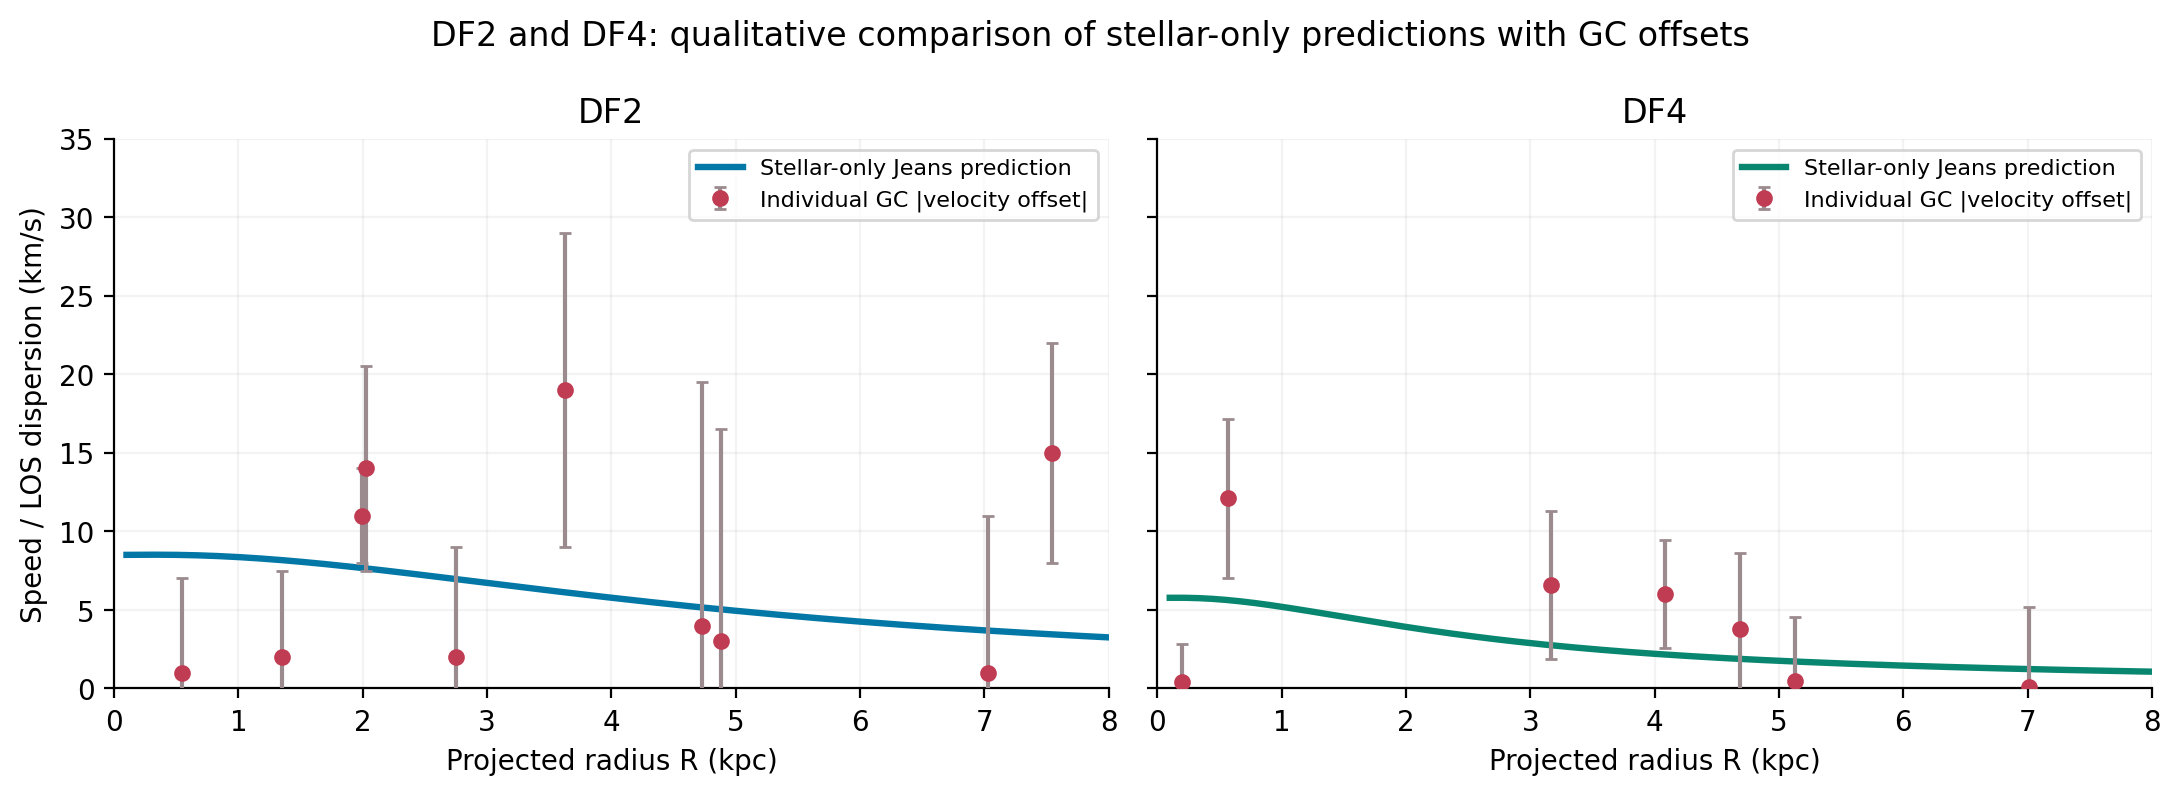
\includegraphics[width=\textwidth]{df2_df4_newtonian.png}
\caption{Calculated stellar-only Newtonian line-of-sight dispersion for DF2 (left) and DF4 (right), compared with absolute line-of-sight velocity offsets of individual globular clusters. Vertical bars show the compiled velocity-measurement uncertainties in a symmetric approximation. Individual offsets are not local estimates of the dispersion. The observational 1$\sigma$, 2$\sigma$, and 3$\sigma$ shaded regions in the source study are not reproduced here.}
\label{fig:df2df4}
\end{figure}

The model curves have the same general declining behaviour as the Newtonian reference curves of Bhatia \emph{et al.} \cite{bhatia2023}. The sparse globular-cluster samples and substantial individual measurement errors limit what can be concluded from a visual overlay. In particular, agreement between the model line and individual absolute velocity offsets is not equivalent to a fitted intrinsic velocity dispersion. The result should be read as a check of the stellar-only Jeans calculation, showing that these models are compatible with the selected data, and not as a measurement of the dark matter content. More recent globular-cluster studies find that the inferred dispersion of these galaxies depends on the membership selection and the adopted distance, so the conclusion is conditional on the data and assumptions used here.

\section{Stellar-Only Models and Anisotropy in DF44}

The DF44 stellar profile has an integrated mass of $2.33\times10^8\,M_\odot$ for the adopted mass-to-light ratio. Figure~\ref{fig:df44stellar} compares the isotropic case with constant radial and tangential anisotropy. The three curves differ most strongly toward the centre and become more similar at larger projected radii. Radial anisotropy ($\beta=0.6$) increases the central projected dispersion relative to the isotropic model; tangential anisotropy ($\beta=-0.6$) lowers it for this stellar profile.

\begin{figure}[htbp]
\centering
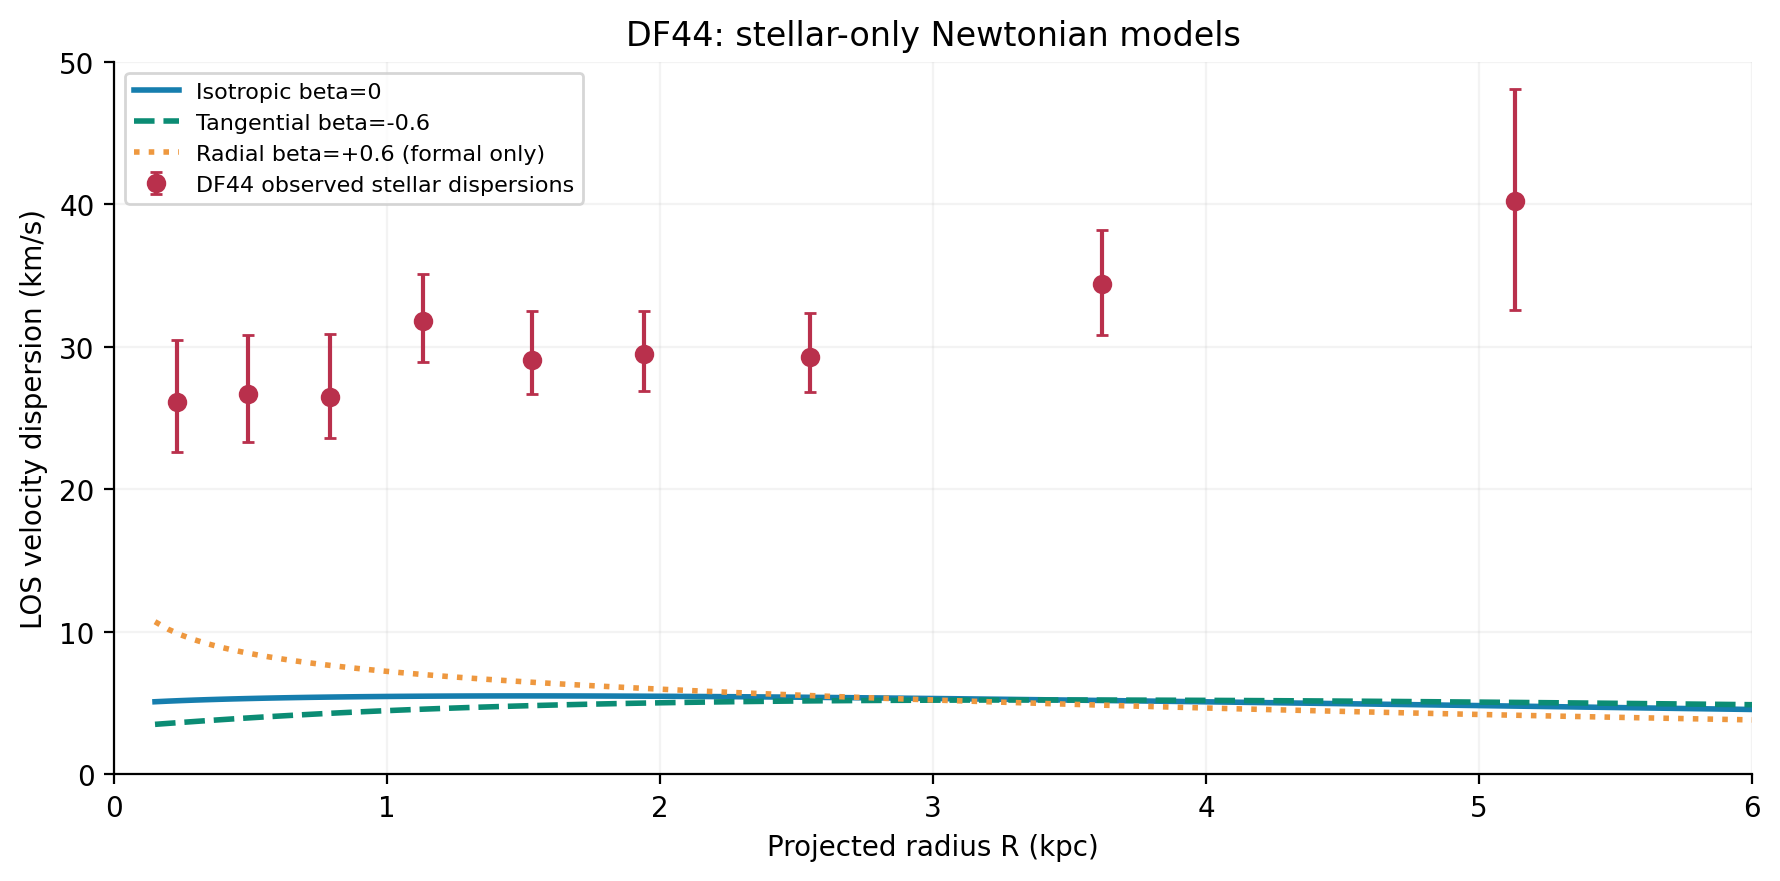
\includegraphics[width=0.95\textwidth]{df44_stellar_only.png}
\caption{DF44 stellar-only Newtonian projections for isotropic ($\beta=0$), radially biased ($\beta=0.6$), and tangentially biased ($\beta=-0.6$) motions. The $\beta=0.6$ curve is a formal Jeans solution that is not physically admissible for this tracer profile (see text). The red data points are the nine spatially resolved stellar velocity dispersions compiled from van Dokkum \emph{et al.} \cite{vandokkumdf44_2019}.}
\label{fig:df44stellar}
\end{figure}

Numerically, and as a fitting exercise, the $\beta=0.6$ curve is a valid solution of Equation~\eqref{eq:jeans}, but physically such a model is not possible. The adopted tracer density rises towards the centre as $r^{-p_n}$ with $p_n\simeq0.41$, so the cusp slope--central anisotropy theorem \cite{anevans2006} requires $\beta_0\le p_n/2\simeq0.21$ at the centre, which a constant $\beta=0.6$ violates. The radial case is therefore retained only as a formal illustration of how radial bias changes the Jeans prediction, and not as a viable model of DF44. The theorem places no restriction on tangential bias, so the tangentially biased curve and the negative-$\beta$ fits below are not affected.

All three stellar-only predictions lie well below the observed DF44 values, which rise from approximately $26\,\mathrm{km\,s^{-1}}$ at small projected radii to approximately $40\,\mathrm{km\,s^{-1}}$ at $R\simeq5.1\,\mathrm{kpc}$ \cite{vandokkumdf44_2019}. At $R=1\,\mathrm{kpc}$ the predicted stellar-only dispersions range from $4.48$ to $7.23\,\mathrm{km\,s^{-1}}$ under the three anisotropy choices. For these tested anisotropies, changing the orbital shape does not close the gap: the amplitude is set largely by the depth of the potential, which the stars alone do not provide. Anisotropy profiles more general than the constant values tried here are not excluded by this calculation, but the size of the shortfall motivates adding a gravitating component that is not visible.

\section{Dark Halo Fit to the DF44 Dispersion Profile}

In the initial illustrative NFW calculation ($M_{200}=7.0\times10^{10}\,M_\odot$, $c=10$, $\beta=-0.8$, $\Upsilon_\star=1\,M_\odot/L_\odot$), the model gives $\chi^2=18.16$ against the nine observed dispersions when evaluated with Equation~\eqref{eq:fitobjective}. We next optimise the halo mass and anisotropy while keeping $c$ and $\Upsilon_\star$ fixed.

The best-fitting conditional parameters are $M_{200}=3.57\times10^{10}\,M_\odot$ and $\beta=-0.6475$, with $\chi^2=4.00$ for $9-2=7$ degrees of freedom, i.e.\ $\chi^2_{\rm red}=0.571$. The fitted dispersion at $R=1\,\mathrm{kpc}$ is $29.18\,\mathrm{km\,s^{-1}}$. As shown in Figure~\ref{fig:df44nfw}, these parameters bring the model much closer to the observations than the initially assumed values. A value of $\chi^2_{\rm red}$ below unity with only nine data points should not be over-interpreted: it is compatible with a good model, with conservative uncertainties, or with small-sample scatter.

\begin{table}[htbp]
 \centering
 \small
 \caption{Independent NFW fits to nine DF44 stellar-dispersion measurements, with $\Upsilon_\star=1\,M_\odot/L_\odot$ fixed. The free-concentration minimum occurs at the imposed bound $c=2$ and should not be treated as a measured halo concentration.}
 \label{tab:df44fits}
 \begin{tabular}{@{}lccccc@{}}
 \toprule
 Fit & $M_{200}\;(10^{10}M_\odot)$ & $c$ & $\beta$ & $\chi^2$ & $\chi^2_{\rm red}$ \\
 \midrule
 Fixed concentration ($k=2$) & 3.57 & 10 (fixed) & $-0.6475$ & 4.00 & 0.571 \\
 Free concentration ($k=3$) & 119.86 & 2 (bound) & $-0.2668$ & 2.92 & 0.487 \\
 \bottomrule
 \end{tabular}
\end{table}

\begin{figure}[htbp]
\centering
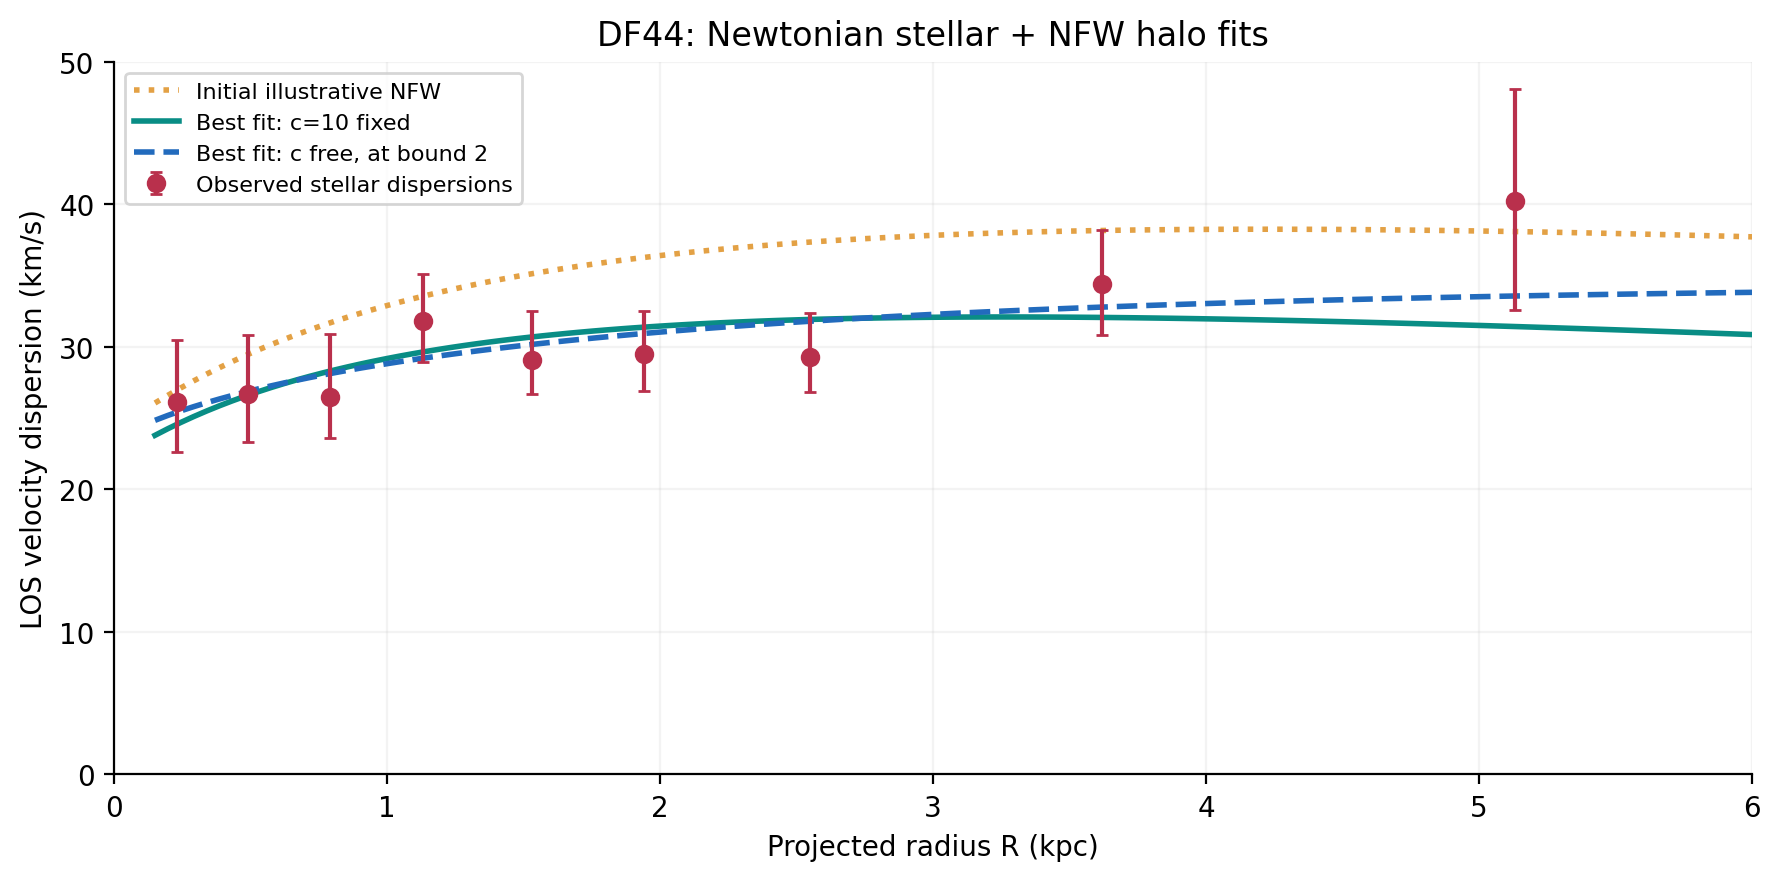
\includegraphics[width=0.96\textwidth]{df44_nfw_bestfit.png}
\caption{DF44 observations with asymmetric error bars compared against the initial illustrative NFW curve and two non-linear least-squares fits. The green line uses $c=10$ with fitted $M_{200}$ and $\beta$. The blue dashed line also fits concentration, but the optimum lies on the lower allowed concentration boundary and is therefore not a unique halo determination.}
\label{fig:df44nfw}
\end{figure}

\subsection*{Dynamical Mass Near the Half-Light Radius}

A simple estimate, independent of the detailed Jeans fit, indicates that DF44 is dark-matter dominated. For a dispersion-supported system, the mass within the three-dimensional half-light radius is approximately $M(<r_{1/2})\simeq3\langle\sigma_{\rm LOS}^2\rangle r_{1/2}/G$ \cite{wolf2010}, where $\langle\sigma_{\rm LOS}^2\rangle$ is the luminosity-weighted mean-square dispersion and $r_{1/2}\simeq4R_e/3\simeq6.3\,\mathrm{kpc}$ for the adopted profile. The luminosity-weighted dispersion reported by van Dokkum \emph{et al.} is about $33\pm3\,\mathrm{km\,s^{-1}}$ \cite{vandokkumdf44_2019}, giving $M(<r_{1/2})\approx4.8\times10^9\,M_\odot$; using the local values $26$ and $40\,\mathrm{km\,s^{-1}}$ as limits gives about $3.0\times10^9$ and $7.0\times10^9\,M_\odot$. The fixed-concentration fit encloses $\approx4.2\times10^9\,M_\odot$ of halo mass plus $\approx1.2\times10^8\,M_\odot$ of stars inside the same radius, within this range. Stars then contribute only a few per cent of the mass, so the dynamical mass exceeds the stellar mass by a factor of order forty. Because the DF44 profile rises with radius and $r_{1/2}$ lies slightly beyond the outermost measured projected radius, this estimate is an order-of-magnitude check and not an independent precision measurement.

\section{Anisotropy, Projection and the Rising Dispersion Profile}

The observed dispersion rises with projected radius, whereas the stellar-only curves decline. Equation~\eqref{eq:los} shows one way in which orbital anisotropy can alter this slope. A line of sight at small $R$ runs nearly parallel to the radius vector and mainly samples $\sigma_r$, whereas at larger $R$ it cuts across orbits and samples tangential motion increasingly. For $\beta<0$ the projection weight $1-\beta R^2/r^2$ exceeds unity and grows with $R/r$, so tangential bias lifts $\sigma_{\rm LOS}$ preferentially at large radius. The halo mass mainly sets the overall level of the curve, while $\beta$ mainly shapes its radial trend. This is a plausible reason for the preference for a tangentially biased solution ($\beta\approx-0.65$), and the sign is consistent with that of $\xi$ reported in the source study. However, changing $\beta$ also changes $\sigma_r(r)$ through the Jeans solution, so the projection factor is only part of the effect, and the cause cannot be established without an anisotropy-only sensitivity test. Constant $\beta$ is also a simplification.

The same reasoning exposes a mass--anisotropy degeneracy, a known limitation of second-moment Jeans modelling: the projected dispersion depends jointly on the potential, which mainly scales the amplitude, and on the orbital structure, which mainly scales the shape, so different pairs of $(M_{200},\beta)$ can produce similar curves over a limited radial range. Nine points with sizeable uncertainties constrain this combination only partially.

\section{Halo Mass Concentration Degeneracy}

When $c$ is allowed to vary over $2\le c\le40$, the minimum reaches $c=2$ with $M_{200}\simeq1.20\times10^{12}\,M_\odot$ and $\beta=-0.267$, giving $\chi^2=2.92$ for six degrees of freedom. Adding the concentration as a free parameter therefore lowers $\chi^2$ by only about $1.1$ (from $4.00$ to $2.92$), which is of the size expected from fitting noise with one extra parameter, and the solution sits on the boundary of the permitted range. It is therefore not a measurement of the concentration.

The reason is physical. The kinematic tracers extend to only a few kpc, whereas $r_{200}$ is tens to hundreds of kpc, so the data constrain the mass enclosed in the region they sample more directly than the halo as a whole. The two solutions enclose almost the same halo mass at $r_{1/2}\simeq6.3\,\mathrm{kpc}$, about $4.2\times10^9\,M_\odot$ in each case, even though $M_{200}$ differs by a factor of about thirty and the scale radius changes from about $6.8\,\mathrm{kpc}$ to about $110\,\mathrm{kpc}$. For the low-concentration solution $r_s$ greatly exceeds the observed radii, so the data sample only the inner $\rho\propto r^{-1}$ cusp and constrain just the product $\rho_s r_s$ (Chapter~2); $M_{200}$ is then an extrapolation of that inner mass to $r_{200}$. A concentration this low is also well below the values typical of halos of this mass in cosmological simulations \cite{dutton2014}; a concentration--mass prior would strongly disfavour it, although it would not by itself exclude it. No confidence intervals are computed here, so the statement that the inner mass is better constrained than $M_{200}$ is qualitative.

\begin{figure}[H]
\centering
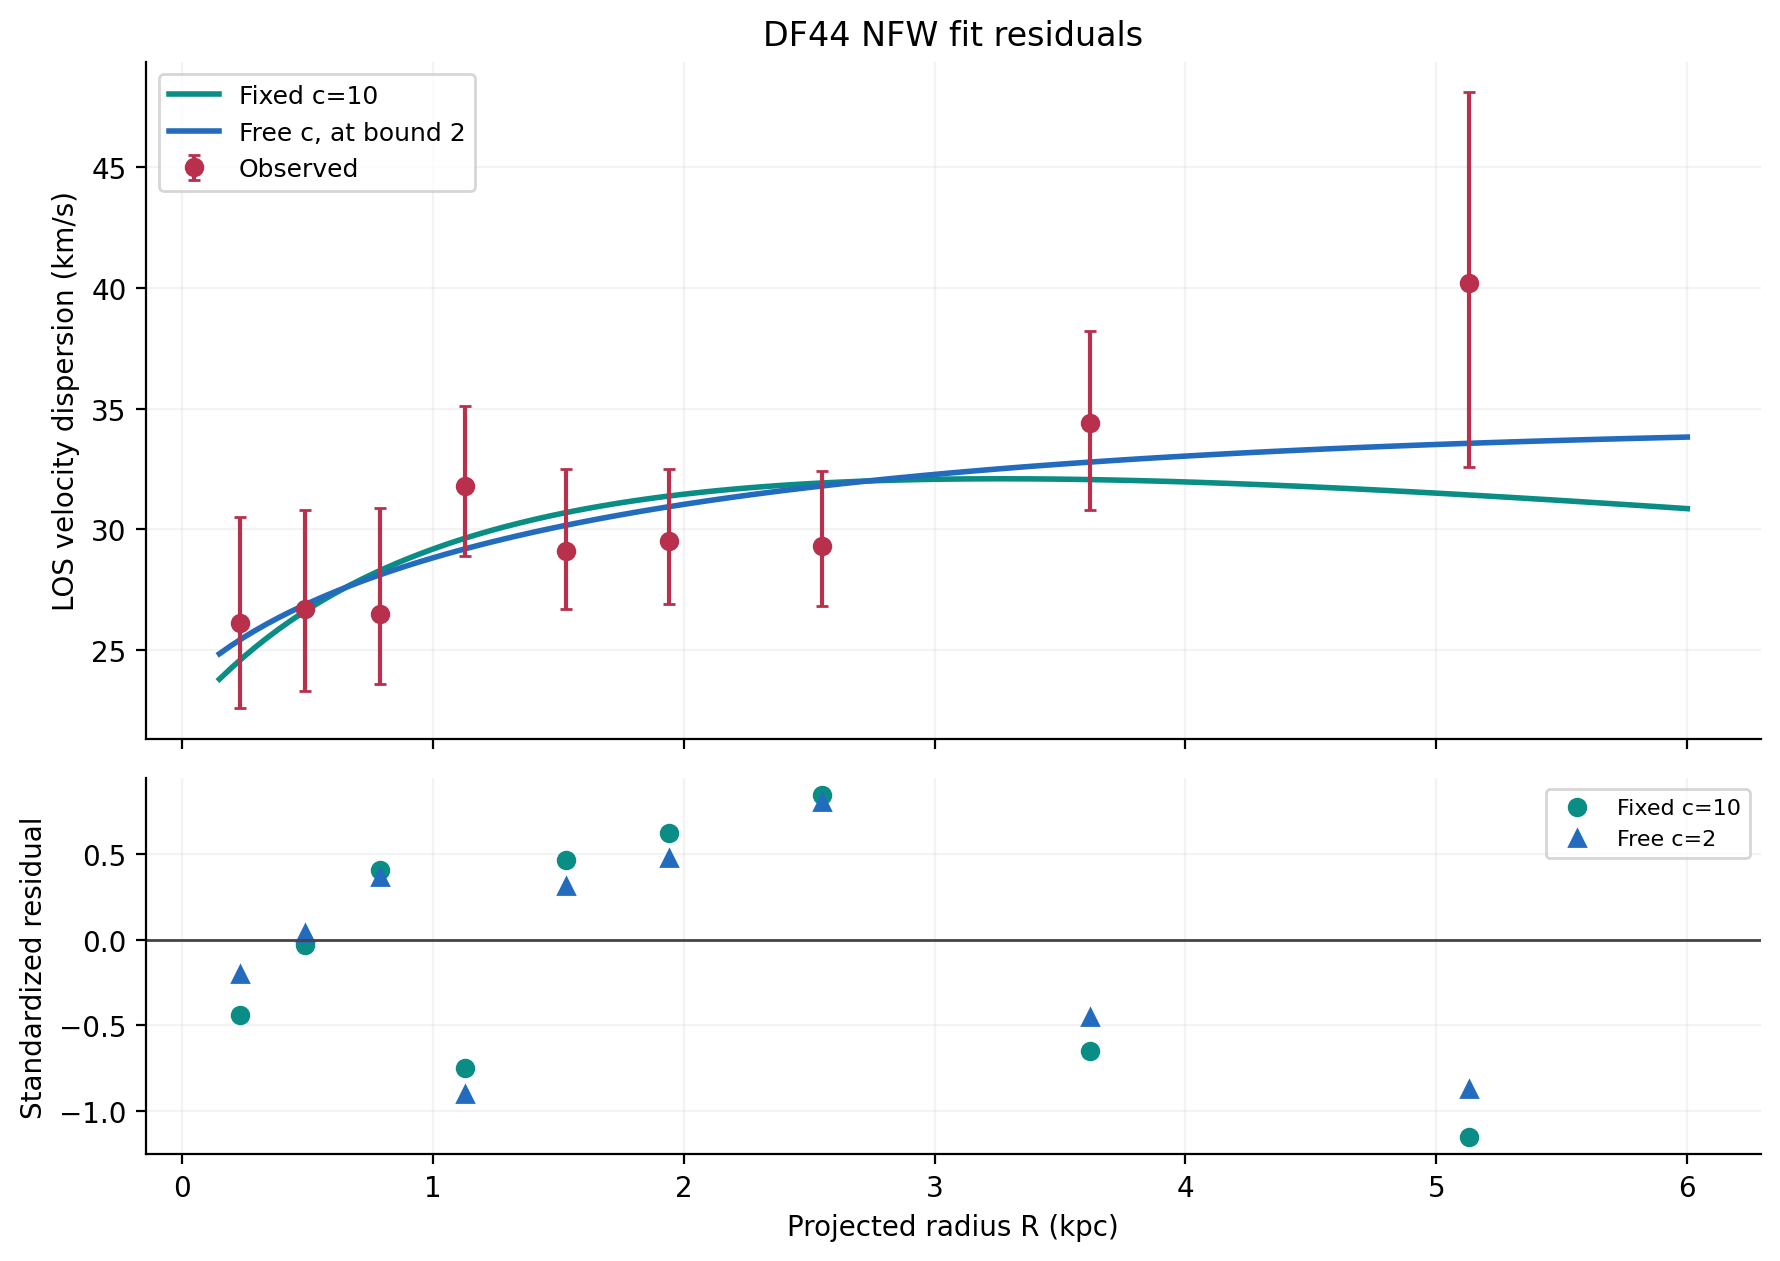
\includegraphics[width=0.88\textwidth]{df44_nfw_fit_residuals.png}
\caption{DF44 NFW fits (top) and standardised velocity-dispersion residuals evaluated with the one-sided uncertainties of Equation~\eqref{eq:spliterrors} (bottom). The residual plot permits inspection of the radial structure left by the fitted models.}
\label{fig:df44residuals}
\end{figure}

\subsection*{Stellar Mass-to-Light Ratio}

A further fit with $c=10$ and variable $\Upsilon_\star$ returns $\Upsilon_\star=0.3\,M_\odot/L_\odot$, again at the imposed lower boundary, with $M_{200}=3.70\times10^{10}\,M_\odot$, $\beta=-0.649$ and $\chi^2=3.98$. The $\chi^2$ falls by only about $0.02$ compared with the two-parameter fit. This follows from the dynamical-mass result above: in this model family stars carry only a few per cent of the mass in the region sampled, so changing their mass-to-light ratio barely changes the potential. This shows that these data and this model do not constrain $\Upsilon_\star$; it is not a statement about what stellar-population methods could achieve.

\subsection*{Comparison with the Published Analysis}

The source study reports $M_{200}\simeq3.98\times10^{10}\,M_\odot$, $\beta\simeq-0.8$ and $\chi^2_{\rm red}\simeq0.75$ for its own NFW model \cite{bhatia2024}. Those results use a concentration--mass relation and a different nuisance-parameter treatment. The numerical proximity of the masses should not be mistaken for an exact replication of the paper's inference, although the agreement in the sign of the anisotropy and the order of magnitude of the halo mass is encouraging.

%===============================================================
\chapter{Conclusions, Limitations and Future Work}
%===============================================================

\section{Conclusions}

Line-of-sight velocity-dispersion profiles of DF2, DF4 and DF44 were computed from spherical stellar-density distributions using the constant-anisotropy Jeans equation and line-of-sight projection. Within the Newtonian, spherical and equilibrium assumptions adopted, the following conclusions are drawn.
\begin{itemize}[leftmargin=1.5em,itemsep=2pt]
 \item For DF2 and DF4, stellar-only Newtonian models reproduce a declining dispersion profile and are compatible with the sparse globular-cluster velocities used, so this comparison does not require a dark matter component. It is a consistency check and not a proof of its absence.
 \item For DF44, stellar-only models fall far below the measured dispersions for the fixed mass-to-light ratio and the three constant anisotropies tested, indicating that the system is dominated by dark matter in the region observed, if Newtonian gravity holds.
 \item A Newtonian stellar-plus-NFW model fitted to the nine published DF44 dispersions describes the data well, with a halo mass of order $10^{10}\,M_\odot$ and a tangentially biased velocity distribution at fixed concentration.
 \item The fit constrains the mass enclosed near the half-light radius more directly than the total halo mass. Halo mass, concentration and anisotropy are partly degenerate, and the free-concentration solution runs to a boundary, so the fitted $M_{200}$ and $\beta$ are conditional estimates and not unique measurements.
\end{itemize}

\section{Limitations}

The results are conditional on a chain of assumptions. The galaxies are treated as spherical, non-rotating systems in dynamical equilibrium with constant anisotropy, and flattening and tidal effects, which may matter for galaxies in groups and clusters, are ignored. A constant anisotropy is also restricted physically: the radial case $\beta=0.6$ used for illustration is not admissible for the adopted tracer cusp, as discussed in Chapter~3. For DF2 and DF4 the observed velocities belong to globular clusters, whose spatial distribution need not follow the stellar light used here as the tracer density, and the comparison uses individual velocity offsets and not local dispersions, with the original confidence bands not reconstructed. The inferred dark matter content of these two galaxies also depends on the adopted distance, on the sparse sampling and, as more recent globular-cluster studies indicate, on the membership selection. The statements about DF2 and DF4 hold only within these assumptions. Likewise, for DF44 the conclusion that stellar-only models fall short holds for the fixed mass-to-light ratio and the anisotropies tested; it does not rule out other mass distributions or gravity theories.

The DF44 fit minimises a piecewise-Gaussian objective and is not the full Bayesian analysis of the source study. The nine measurements are treated as independent, and aperture and seeing effects are approximated by evaluating the model at representative radii. The tabulated dispersions are used directly, although the source figure plots an effective dispersion that also includes the mean velocity; the difference is small for DF44. No concentration--mass prior is imposed, and the free-concentration solution lies on a parameter boundary, so the fitted values of $M_{200}$ and $\beta$ are conditional estimates. No confidence intervals are computed, which means that statements about which quantities are better constrained are qualitative. The half-light mass estimate is an order-of-magnitude check, and only the Newtonian baselines of the source papers are implemented.

\section{Future Work}

Three extensions follow naturally from this work. First, the least-squares fit can be replaced by Bayesian inference, for example MCMC sampling with a cosmological concentration--mass prior. This would give credible intervals on the halo mass, concentration and anisotropy and would down-weight values such as the boundary solution found here, although the intervals will still depend on the priors, and sampling alone does not remove the mass--anisotropy degeneracy. Second, the analysis can be extended to the modified-gravity models discussed in the source papers, so that Newtonian-plus-halo and modified-gravity descriptions can be compared on the same data; such a comparison shows which description fits better, but does not by itself provide independent evidence for any one theory. Third, other dark matter profiles can be tested, in particular cored halos, which van Dokkum \emph{et al.} found able to describe DF44 with nearly isotropic orbits \cite{vandokkumdf44_2019}, to examine how sensitive the inferred halo and anisotropy are to the assumed inner density profile.

%---------------------------------------------------------------
\clearpage
\addcontentsline{toc}{chapter}{References}
\begin{thebibliography}{99}
\bibitem{bhatia2023}
E. Bhatia, S. Chakrabarti, and S. Chakraborty,
``Velocity dispersion of dark-matter deficient ultradiffuse galaxies: A case for modified gravity,''
\emph{Physical Review D} \textbf{108}, 064021 (2023).
\url{https://doi.org/10.1103/PhysRevD.108.064021}.

\bibitem{bhatia2024}
E. Bhatia, S. Chakrabarti, and S. Chakraborty,
``Exploring velocity dispersion anisotropy in a dark matter dominated ultra-diffuse galaxy with modified gravity models,''
\emph{Physical Review D} \textbf{112}, 024034 (2025), arXiv:2412.03658.
\url{https://doi.org/10.1103/2k1h-fj16}.

\bibitem{vandokkum2018}
P. van Dokkum \emph{et al.},
``A galaxy lacking dark matter,''
\emph{Nature} \textbf{555}, 629--632 (2018).
\url{https://doi.org/10.1038/nature25767}.

\bibitem{vandokkumdf4_2019}
P. van Dokkum, S. Danieli, R. Abraham, C. Conroy, and A. J. Romanowsky,
``A second galaxy missing dark matter in the NGC1052 group,''
\emph{The Astrophysical Journal Letters} \textbf{874}, L5 (2019).
\url{https://doi.org/10.3847/2041-8213/ab0d92}.

\bibitem{vandokkumdf44_2019}
P. van Dokkum \emph{et al.},
``Spatially resolved stellar kinematics of the ultra-diffuse galaxy Dragonfly 44. I. Observations, kinematics, and cold dark matter halo fits,''
\emph{The Astrophysical Journal} \textbf{880}, 91 (2019).
\url{https://doi.org/10.3847/1538-4357/ab2914}.

\bibitem{navarro1997}
J. F. Navarro, C. S. Frenk, and S. D. M. White,
``A universal density profile from hierarchical clustering,''
\emph{The Astrophysical Journal} \textbf{490}, 493--508 (1997).
\url{https://doi.org/10.1086/304888}.

\bibitem{binney2008}
J. Binney and S. Tremaine,
\emph{Galactic Dynamics}, 2nd ed. (Princeton University Press, 2008).

\bibitem{mamon2005}
G. A. Mamon and E. L. \L{}okas,
``Dark matter in elliptical galaxies: II. Estimating the mass within the virial radius,''
\emph{Monthly Notices of the Royal Astronomical Society} \textbf{363}, 705--722 (2005).
\url{https://arxiv.org/abs/astro-ph/0405491}.

\bibitem{wolf2010}
J. Wolf \emph{et al.},
``Accurate masses for dispersion-supported galaxies,''
\emph{Monthly Notices of the Royal Astronomical Society} \textbf{406}, 1220--1237 (2010).

\bibitem{anevans2006}
J. An and N. W. Evans,
``A cusp slope--central anisotropy theorem,''
\emph{The Astrophysical Journal} \textbf{642}, 752 (2006).
\url{https://arxiv.org/abs/astro-ph/0511686}.

\bibitem{dutton2014}
A. A. Dutton and A. V. Macci\`o,
``Cold dark matter haloes in the Planck era: evolution of structural parameters for Einasto and NFW profiles,''
\emph{Monthly Notices of the Royal Astronomical Society} \textbf{441}, 3359 (2014).
\url{https://arxiv.org/abs/1402.7073}.
\end{thebibliography}
\end{document}
